\documentclass[12pt]{article}
\usepackage[utf8]{inputenc}
\usepackage[spanish]{babel}
\usepackage{ragged2e}
\usepackage{amsmath}
\usepackage{graphicx}
\usepackage{hyperref}
\usepackage{fancyhdr}
\usepackage{subcaption}
\usepackage{listings}
\usepackage{color}

\definecolor{dkgreen}{rgb}{0,0.6,0}
\definecolor{gray}{rgb}{0.5,0.5,0.5}
\definecolor{mauve}{rgb}{0.58,0,0.82}

\lstset{frame=tb,
  language=Python,
  aboveskip=3mm,
  belowskip=3mm,
  showstringspaces=false,
  columns=flexible,
  basicstyle={\small\ttfamily},
  numbers=none,
  numberstyle=\tiny\color{gray},
  keywordstyle=\color{blue},
  commentstyle=\color{dkgreen},
  stringstyle=\color{mauve},
  breaklines=true,
  breakatwhitespace=true,
  tabsize=3
}

\title{\huge Práctica Supervisada\vspace*{5cm}}

\author{Amallo, Sofía - Gil, Juan Manuel}

\date{\parbox{\linewidth}{\centering%
  Noviembre 18, 2022 \endgraf\bigskip
  \vspace*{4cm}
  Dr. Ing. Horacio A. Mendoza \hspace*{1cm} Dr. Ing. Jorge Finochietto\endgraf\medskip
  \vspace*{0.5cm}
  Laboratorio de\ Comunicaciones Digitales \endgraf
  Universidad Nacional de Córdoba}}
  
\begin{document}

\maketitle
\thispagestyle{empty}
\newpage

%\pagestyle{myheadings}
\markright{}

\section{Ficha de Práctica Supervisada}
\subsection{Datos de los Alumnos}
\raggedright
\textsl{Nombre y Apellido:}  Sofía Amallo

\textsl{N° de Matrícula:} 41.279.731

\textsl{Teléfono:} (+54) 351 2355718

\textsl{Correo electrónico:} sofia.amallo@mi.unc.edu.ar
\vspace*{0.5cm}

\textsl{Nombre y Apellido:} Juan Manuel Gil

\textsl{N° de Matrícula:} 41.592.940

\textsl{Teléfono:} (+54) 3571 604632

\textsl{Correo electrónico:} juan.manuel.gil@mi.unc.edu.ar

\subsection{Datos de la Institución Receptora}
\textsl{Nombre:} Laboratorio de Comunicaciones Digitales

\textsl{Dirección del Laboratorio:} Av. Vélez Sársfield 1600 CU, Cba - Argentina

\textsl{Nombre y Apellido del Supervisor Docente:} Dr. Ing. Jorge Manuel Finochietto

\textsl{Cargo que ocupa el Supervisor Docente en la Institución Receptora:} Secretario de Tecnología  Educación Virtual, Jefe de cátedra de Informática e Investigador Independiente del CONICET

\textsl{N° de Teléfono:} (+54) 351 5353800 int 29085

\textsl{Correo Electrónico:} lcd@fcefyn.unc.edu.ar

\subsection{Datos del Tutor}

\textsl{Nombre y Apellido:} Dr. Ing. Horacio A. Mendoza

\textsl{Cargo y Cátedra:} Docente e Investigador

\textsl{Teléfono:} (+54) 351 5353800 int 29085

\textsl{Correo Electrónico:} lcd@fcefyn.unc.edu.ar

\subsection{Datos de la Práctica Profesional Supervisada}

\textsl{Fecha de Inicio:} 26/09/2022

\textsl{Fecha de Finalización:} 18/11/2022

\textsl{Total de horas:} 222

\tableofcontents
\newpage

\justifying
\section{Resumen}
\setlength\parindent{24pt}
\newpage
\section{Introducción}
La Práctica Supervisada (PS) se llevó a cabo en el Laboratorio de Comunicaciones Digitales (LCD) de la Universidad Nacional de Córdoba, Córdoba, Argentina, donde se abordó el desafío de desarrollar \textit{payloads}, tam-bién conocidas como cargas útiles, con el fin de expandir las funcionalidades del drone Matrice 300 RTK de DJI.

En ese contexto se investigaron distintas maneras de interactuar con dicho drone, siendo algunas, el SDK (Software Development Kit) el cual es brindado por el fabricante y cumple el rol de una API (Application Programming Interface). Se investigó acerca del protocolo UART como solución al problema de la comunicación entre el drone y las distintas payloads.

Una de las partes mas enriquecedoras de nuestra experiencia en el labora-torio fue la dinámica de trabajo, ya que abordamos diferentes soluciones a medida que se presentaron nuevas problemáticas, algo propio del desarrollo con nuevas tecnologías como es nuestro caso. 

La curva de aprendizaje en dichas tecnologías se documentó en Notion, una plataforma de sofware orientada a la toma de notas, lo cual nos permitirá confeccionar de una manera concisa una llamada ``hoja de ruta"  que quede a disposición de otros estudiantes que transiten por el LCD, con el objetivo de brindarle alguna retribución a la institución que nos brindó herramientas de trabajo, acceso a equipos, placas e insumos para el desarrollo de nuestro trabajo y sobre todo un espacio de aprendizaje junto a docentes y compañeros. Sin dudas nuestro paso por el Laboratorio de Comunicaciones Digitales se constituyó en una de las experiencias fundamentales de nuestra formación en el campo profesional.

\vspace{1.5cm}
\begin{tabular}{p{5.5cm}cp{5.5cm}}
  \cline{1-1} \cline{3-3} \\
  \centering Estudiante   \\ Sofía, Amallo && \centering Estudiante \\ Gil, Juan Manuel
\end{tabular}

\vspace{1.5cm}

\begin{tabular}{p{5.5cm}cp{5.5cm}}
  \cline{1-1} \cline{3-3} \\
  \centering Supervisor   \\ Dr. Ing. Finochietto, Jorge M. && \centering Tutor \\ Dr. Ing. Mendoza, Horacio A.
\end{tabular}


\newpage
\section{Herramientas de trabajo}
\justifying
Para realizar las experiencias, que se describirán posteriormente en este documento, fueron necesarias algunas placas de desarrollo, las mismas se listarán en esta sección.
\subsection{PyCom}
Por un lado se utilizó hardware del fabricante \textit{PyCom}, en particular, los módulos \textit{FiPy}[Fig. 4.1 y Fig. 4.2] y su placa de expansión \textit{FyPy}[Fig. 4.3 y Fig 4.4]. La utilización de estas placas fue debido a que se proyecta que las futuras payloads que lleve el drone sean estas o similares.

\begin{figure}[ht]
  \centering
  \begin{subfigure}[b]{0.45\linewidth}
    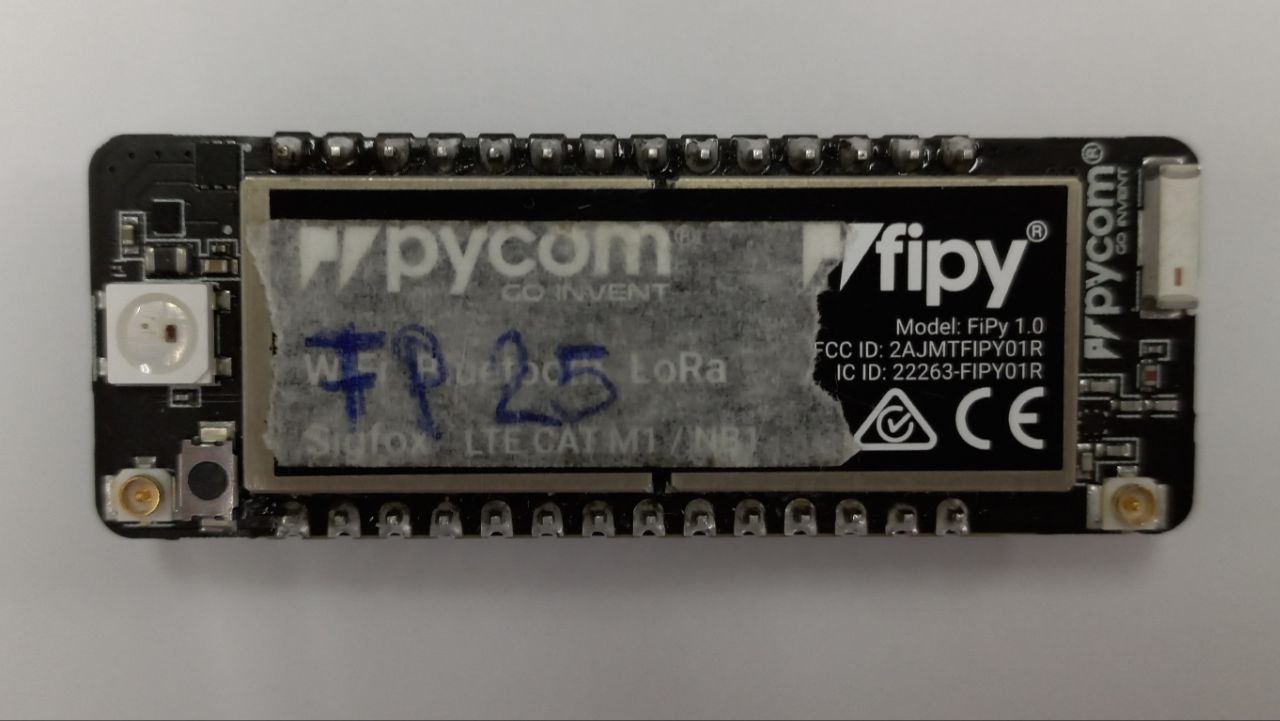
\includegraphics[width=\linewidth]{images/FiPy-1.jpg}
    \caption{Fig. 4.1: FiPy frente}
    \label{fig:FiPy-fte}
  \end{subfigure}
  \begin{subfigure}[b]{0.45\linewidth}
    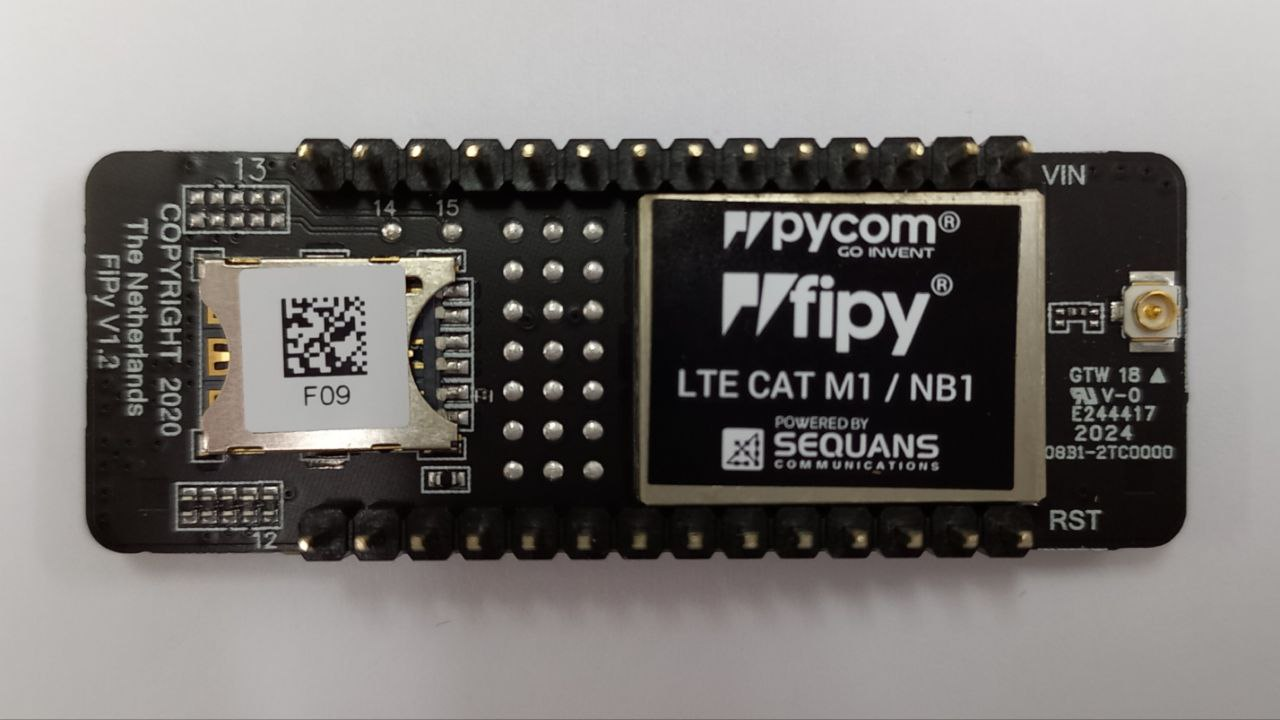
\includegraphics[width=\linewidth]{images/FiPy-2.jpg}
    \caption{Fig. 4.2: FiPy dorso}
    \label{fig:FyPy-dor}
  \end{subfigure}
  \centering
  \begin{subfigure}[b]{0.45\linewidth}
    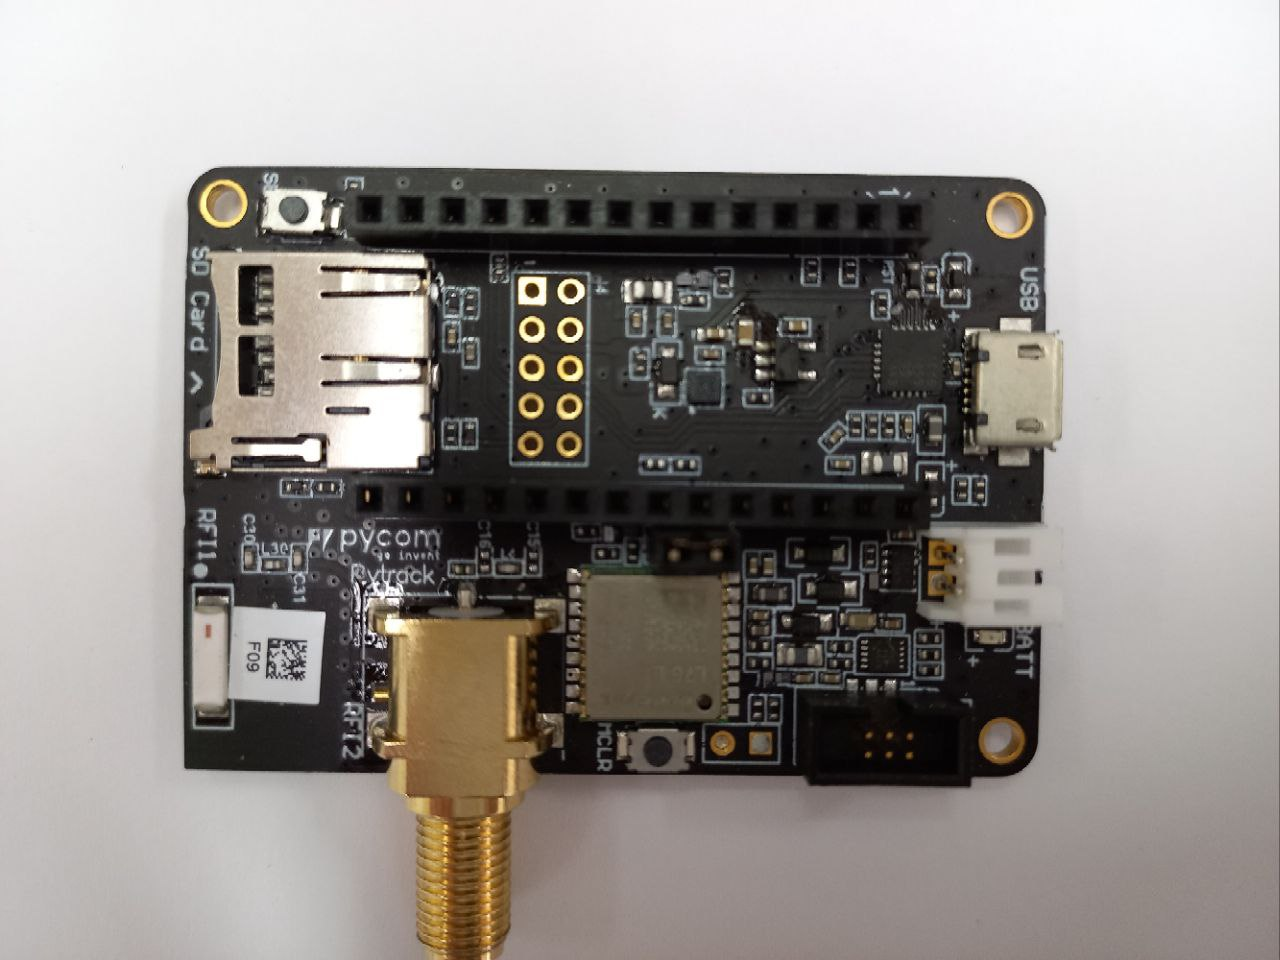
\includegraphics[width=\linewidth]{images/PyTrack-1.jpg}
    \caption{Fig. 4.3: PyTrack frente}
    \label{fig:PyTrack-fte}
  \end{subfigure}
  \begin{subfigure}[b]{0.45\linewidth}
    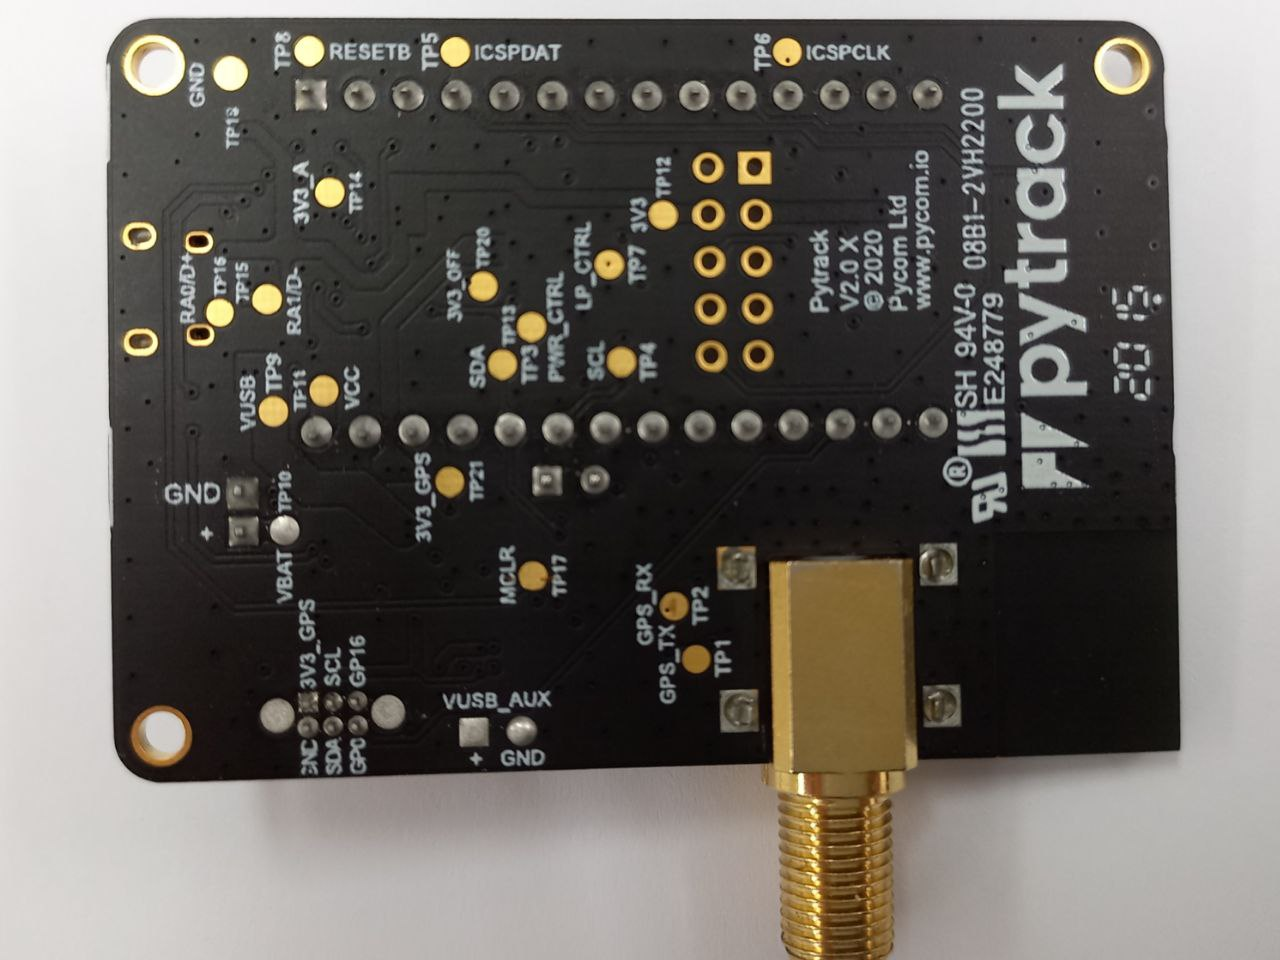
\includegraphics[width=\linewidth]{images/PyTrack-2.jpg}
    \caption{Fig. 4.4: PyTrack dorso}
    \label{fig:PyTrack-dor}
  \end{subfigure}
\end{figure}

Las \textit{PyCom} pueden trabajar con distintos módulos fábricados por terceros a través de sus pines GPIO, o utilizando sus puertos UART. También son capaces de brindar interfaces de red tales como WiFi, Bluetooth, Celular, Lora y Sigfox.

En cuanto a procesamiento cuenta con una \textit{ESP32 SoC} lo que implica un microprocesador Xtensa, con arquitectura ARM de 32-bits; dual-core, con una frecuencia de trabajo de 240MHz.

Una lista completa con todas las funcionalidades ofrecidas por los módulos puede ser consultada en el \href{https://docs.pycom.io/gitbook/assets/specsheets/Pycom_002_Specsheets_FiPy_v2.pdf}{manual de usuario de FiPy} y/o el \href{https://pycom.io/product/pytrack-2-0-x/}{manual de usuario de PyTrack}.

Ambas placas utilizan el lenguaje \href{https://github.com/micropython/micropython}{micropython} para el desarrollo, el cual es un set de funciones reducidas de los módulos originales de Python.

\subsection{SMT32F4}
Esta placa se utilizó con el objetivo de realizar pruebas tratándola como una interfaz drone-payloads, el plan era consumir del SDK del drone (escrito en c) y pasarle información a la \textit{PyCom}, al igual que, en base a los datos recopilados por la payload, darle instrucciones al UAV.
La \textit{SMT32F4} [Fig. 4.5, 4.6] es una placa que posee un procesador Cortex M4, con arquitectura ARM de 32-bit y una frecuencia de operación de 180 MHz. Nos brinda múltiples GPIO para la interacción con hardware y sensores de terceros. Si requiere indagar un poco más sobre la placa puede consultar su \href{https://drive.google.com/file/d/182H9i1qmJ2UCbynztxymEA3nfmx_eGrk/view?usp=share_link}{\textit{manual}}.

\begin{figure}[ht]
  \centering
  \begin{subfigure}[b]{0.45\linewidth}
    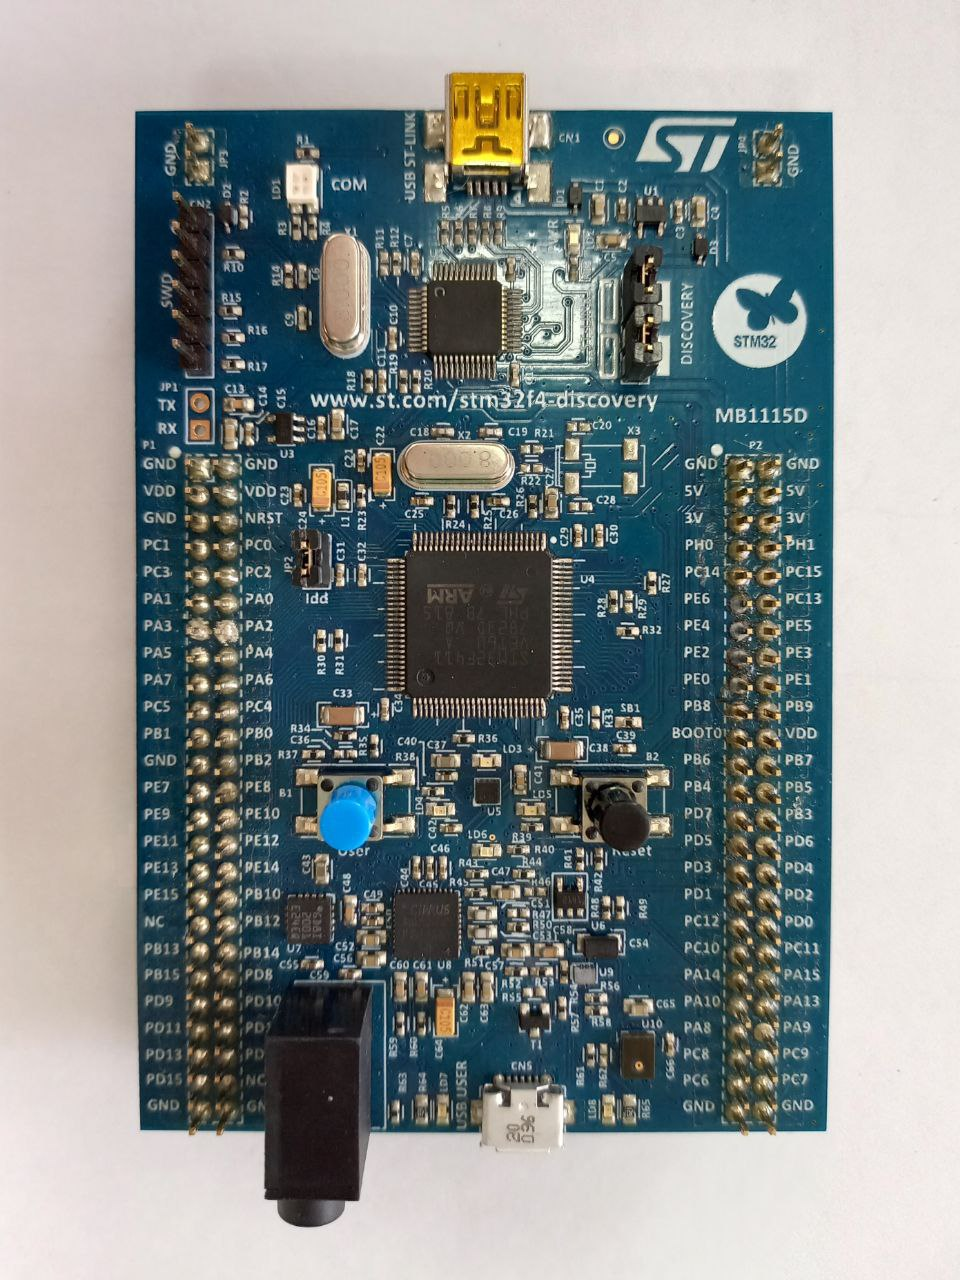
\includegraphics[width=\linewidth]{images/STM32F4-1.jpg}
    \caption{Fig. 4.5: STM32F4 frente}
  \end{subfigure}
  \begin{subfigure}[b]{0.45\linewidth}
    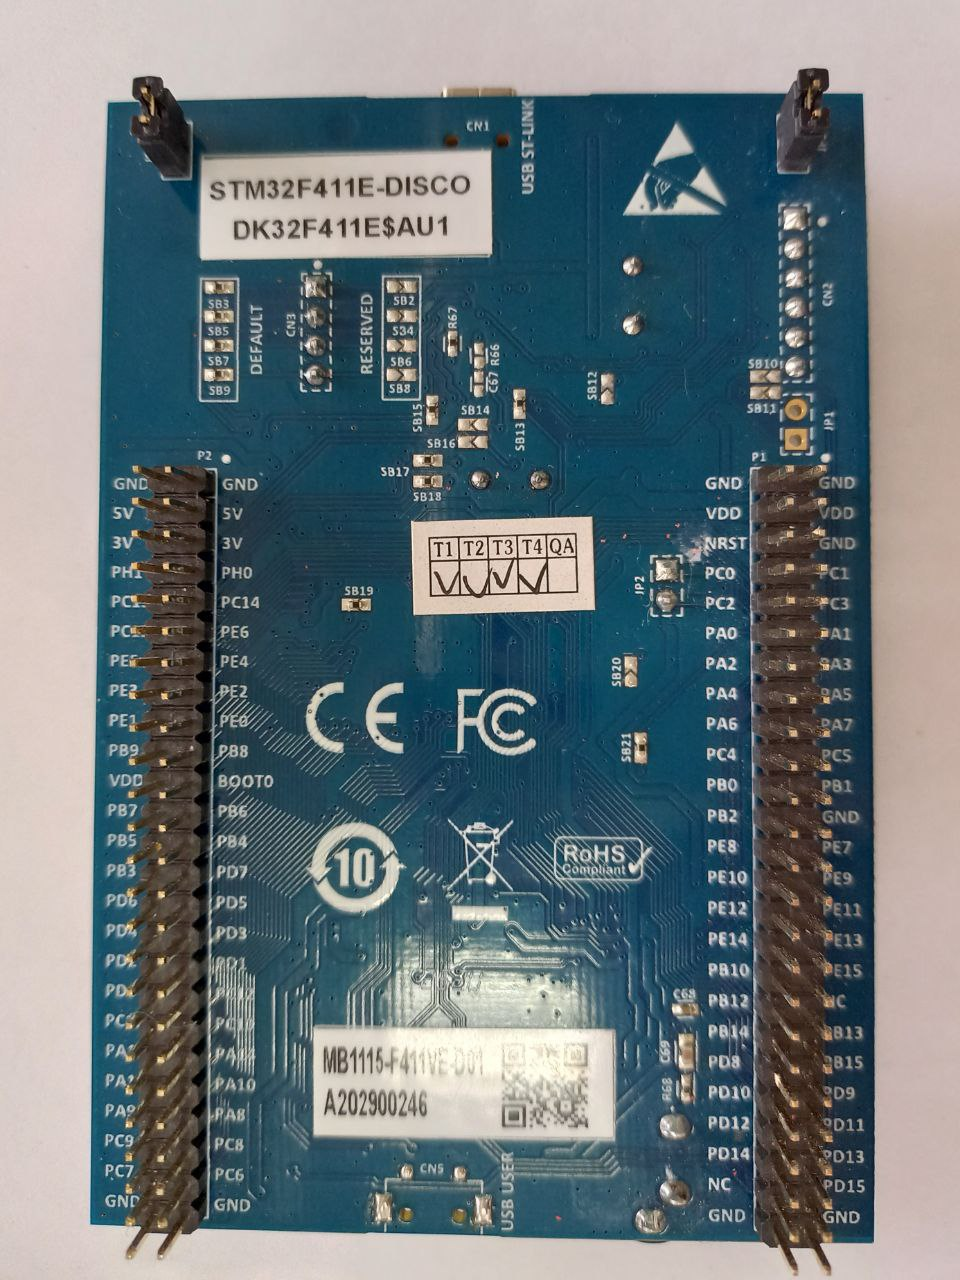
\includegraphics[width=\linewidth]{images/STM32F4-2.jpg}
    \caption{Fig. 4.6: STM32F4 dorso}
  \end{subfigure}
\end{figure}


\subsection{USB to UART}
Este adaptador se utilizó en instancias de pruebas para poder enviar datos desde la PC a las placas, o recibir desde las placas a la PC.

\begin{figure}[ht]
  \centering
  \begin{subfigure}[b]{0.45\linewidth}
    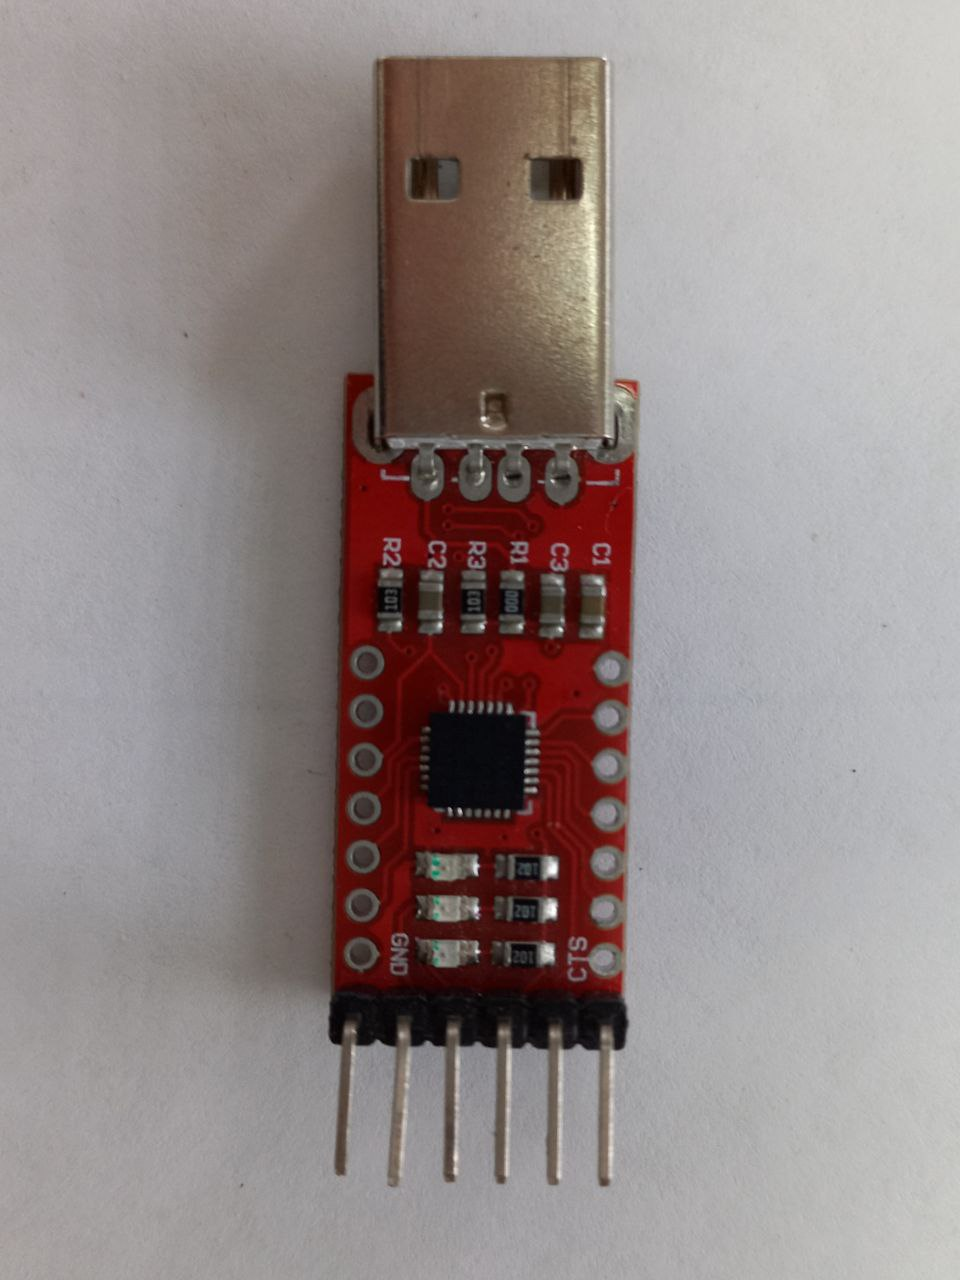
\includegraphics[width=\linewidth]{images/USB-UART-1.jpg}
    \caption{Fig. 4.7: USB to UART frente}
  \end{subfigure}
  \begin{subfigure}[b]{0.45\linewidth}
    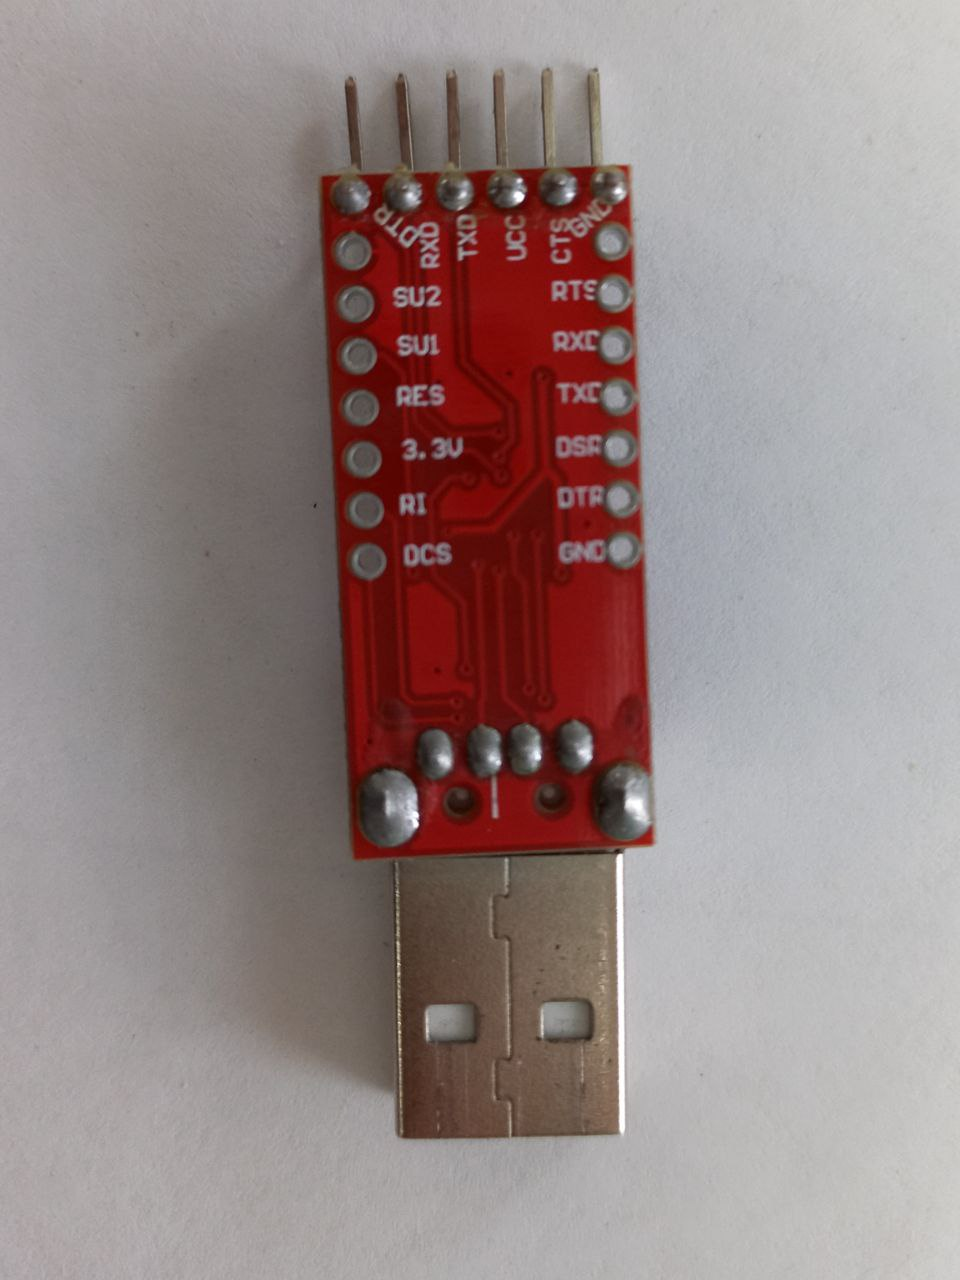
\includegraphics[width=\linewidth]{images/USB-UART-2.jpg}
    \caption{Fig. 4.8: USB to UART dorso}
  \end{subfigure}
\end{figure}

\subsection{Payload SDK Devekopment Board Kit}
La utilización de la \textit{SMT32F4} se debió a que en un primer momento no se tuvo en cuenta que el drone ya contaba con un accesorio para realizar esta tarea, la \href{https://store.dji.com/product/psdk-development-kit}{\textit{Payload SDK Devekopment Board Kit}} [Fig. 4.5, Fig. 4.6 y 4.7]
Luego de investigaciones vimos que esto es justo lo que se precisaba, ya que nos brinda una interfaz para la conexión con el drone, y una placa de desarrollo la cual también es una \textit{SMT32} con un pocesador ARM de 32-bit, no se cuenta con más detalles de dicho chip, aún así debería cubrir todas las interacciones con el SDK de DJI.

\begin{figure}[ht]
  \centering
  \begin{subfigure}[b]{0.45\linewidth}
    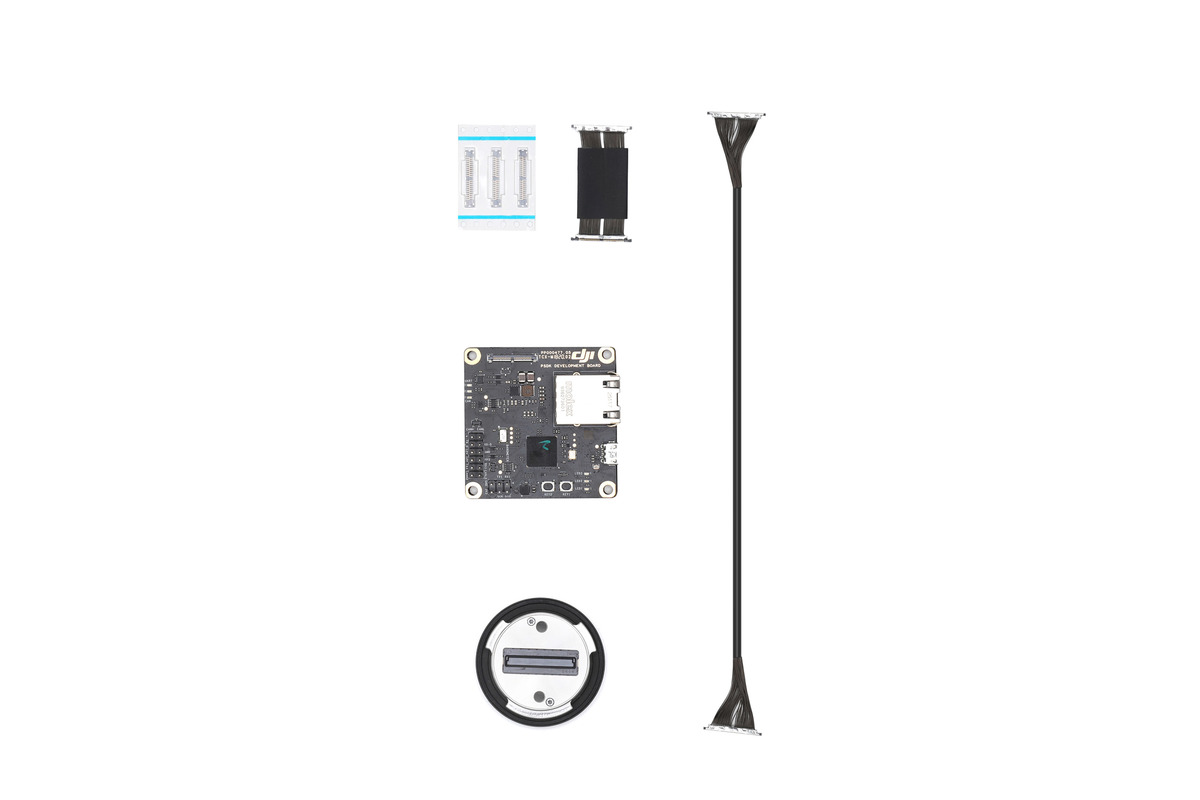
\includegraphics[width=\linewidth]{images/Payload-DBK-1.jpg}
    \caption{Fig. 4.9: kit completo}
  \end{subfigure}
  \begin{subfigure}[b]{0.45\linewidth}
    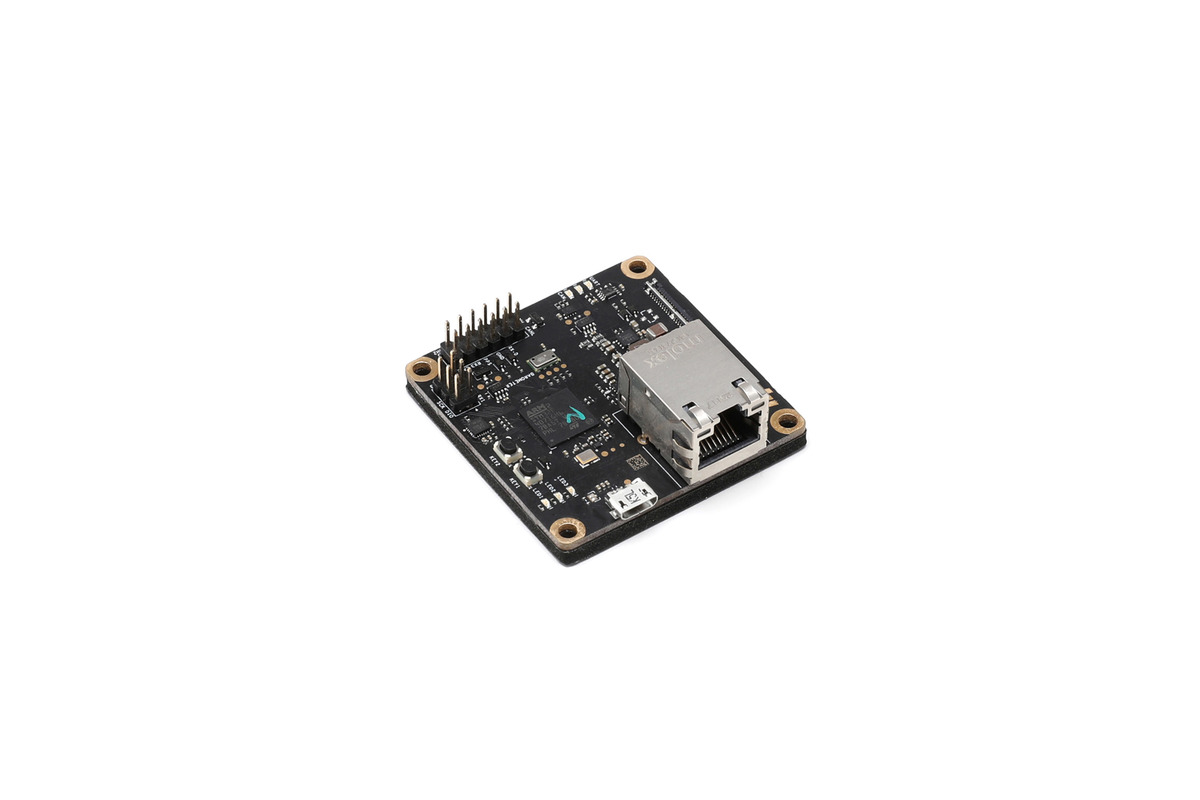
\includegraphics[width=\linewidth]{images/Payload-DBK-2.jpg}
    \caption{Fig. 4.10: Placa de desarrollo}
  \end{subfigure}
  \begin{subfigure}[b]{0.45\linewidth}
    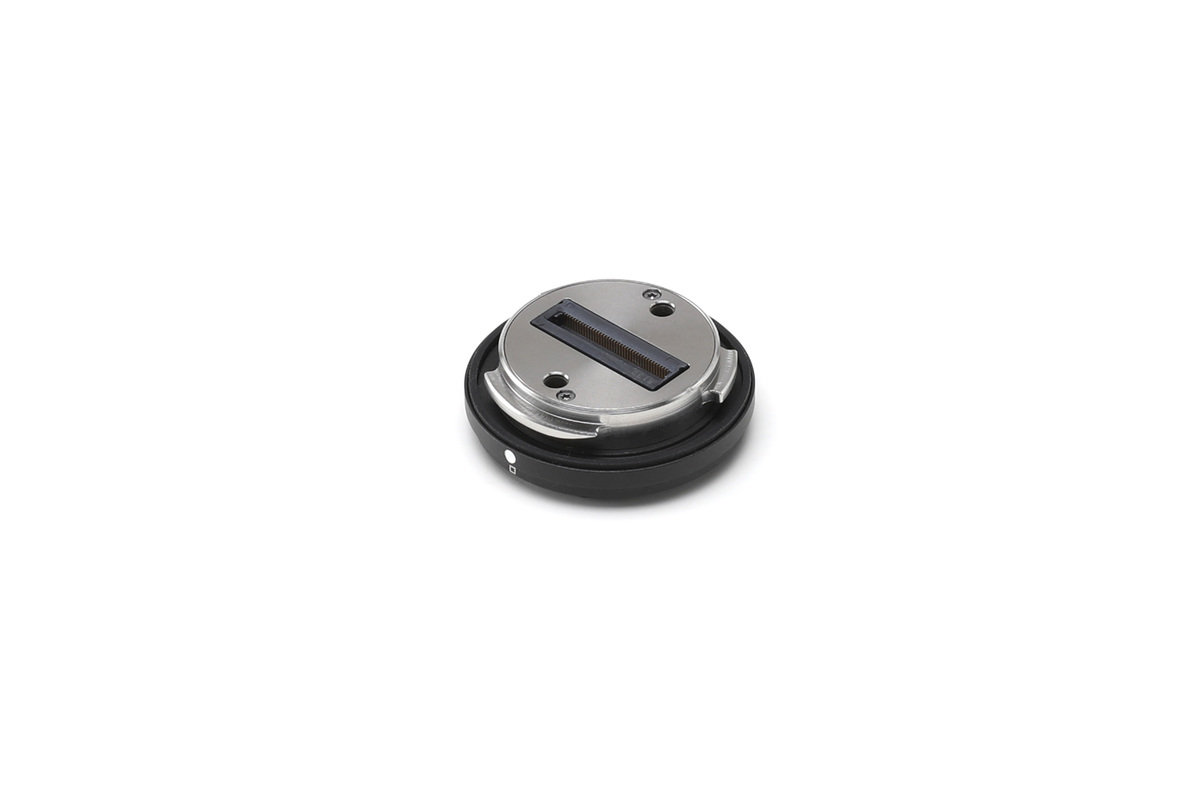
\includegraphics[width=\linewidth]{images/Payload-DBK-3.jpg}
    \caption{Fig 4.11: Conector de la interfaz}
  \end{subfigure}
\end{figure}

\vspace*{200pt}
\newpage
\section{Desafíos abordados}

\subsection{Transmisión datos entre SMT32 y PyCom}
Mientras se analizaban las distintas alternativas para interactuar entre el \textit{SDK del drone} y la payload se hicieron pruebas para que sea una placa \textit{SMT32} la que se conecte directamente al \textit{Matrice 300 RTK} mientras que sea la \textit{PyCom} la que se encargue de  realizar el trabajo útil. Para que esto funcione necesitabamos definir un protocolo de comunicación entre ambas placas, por lo que se optió por utilizar \textit{UART} como medio de transmisión de datos.

\subsubsection{Protocolo UART}
UART significa universal asynchronous receiver/transmitter y define un protocolo, o una serie de reglas, para intercambiar datos de manera serial entre dos dispositivos. Este protocolo es muy simple y utiliza solamente dos cables entre el transmisor y el receptor para enviar y recibir en ambas direcciones. Ambos terminales deben tener una conexión a tierra. 

Una de las grandes ventajas del UART es que es asíncrono: el transmisor y el receptor no comparten una señal de reloj común. Aunque esto simplifica enormemente el protocolo, pone ciertos requisitos al transmisor y al receptor. Dado que no comparten un reloj, ambos terminales deben transmitir a la misma velocidad preestablecida para que tengan la misma sincronización de bits. Las velocidades de baudios del UART más comunes que se utilizan en estos días son 4800, 9600, 19.2K, 57.6K y 115.2K, en nuestro caso se usó 9600. Además de tener la misma velocidad en baudios, ambos lados de una conexión UART también deben utilizar los mismos parámetros y estructura de trama. \cite{uart}

La comunicación UART puede ser simplex(los datos son enviados solo en una dirección), half-duplex(los datos pueden ser enviados en ambas direcciones pero no al mismo tiempo) o full-duplex(los datos pueden ser enviados en ambas direcciones al mismo tiempo).

\subsubsection{Programacion del modulo UART de la SMT32F4}
Para poder utilizar el modulo UART de la \textit{SMT32F4} es necesario realizar una configuración previa. Se utilizó la librería \texttt{UART HAL} que nos brinda el fabricante de la placa. 

El modulo nos permite realizar la comunicación de manera asíncrona o síncrona. En nuestro caso se optó por hacerlo de manera asíncrona. Además, se utilizó el método de polling, o bloqueante, para evitar el uso de interrupciones. 

La librería \texttt{UART HAL} posee una estructura llamada \texttt{UART\_InitTypeDef} que inicializa los parámetros del módulo.

\begin{lstlisting}[language=C]
  typedef struct
{
  uint32_t BaudRate; /* Configura el baud_rate del modulo. */

  uint32_t WordLength; /* Especifica la cantidad de bits recibidos o transmitidos en un frame. */

  uint32_t StopBits; /* Especifica la cantidad de bits de stop. */

  uint32_t Parity; /* Indica la paridad */

  uint32_t Mode; /* Modo recepcion o transmision */

  uint32_t HwFlowCtl;  /* Indica si se utiliza el control de flujo hardware */

  uint32_t OverSampling; /* Indica si se utiliza oversampling */
} UART_InitTypeDef;

\end{lstlisting}

Otra estructura importante que se usó para configurar el modulo es la \texttt{UART\_HandleTypeDef} que se encarga de configurar otros parámetros como los códigos de error, los puteros a los buffers de datos, el tamaño de los mismos, etc.


Para inicializar el modulo se debe llamar a la función \texttt{HAL\_UART\_Init} y pasarle como parámetro la estructura \texttt{UART\_HandleTypeDef}. 
\\\\
\lstinline|HAL_StatusTypeDef HAL_UART_Init(UART_HandleTypeDef *huart)|
\\\\
Para la transmisión se utiliza la función transmit:
\\\\
\lstinline|HAL_StatusTypeDef HAL_UART_Transmit(UART_HandleTypeDef *huart, uint8_t *pData, uint16_t Size, uint32_t Timeout)|
\\\\
Donde el primer parámetro es un puntero a una estructura \texttt{UART\_HandleTypeDef} que contiene información sobre la configuración del módulo, el segundo parámetro es un puntero a un buffer de datos que se desea transmitir, el tercer parámetro es la cantidad de datos (u8 o u16) a transmitir y el cuarto parámetro es el tiempo de espera para reintentar el envio. Esta función retorna un valor de tipo \texttt{HAL\_StatusTypeDef} que es un enum que contiene el estado( \texttt{HAL\_OK, HAL\_ERROR, HAL\_BUSY o HAL\_TIMEOUT}).

Para la recepción se utiliza la función receive:
\\\\
\lstinline|HAL_StatusTypeDef HAL_UART_Receive(UART_HandleTypeDef *huart, uint8_t *pData, uint16_t Size, uint32_t Timeout)|
\\\\
Muchos de los parámetros son los mismos que los mencionados anteriormente, con la diferencia que el segundo parámetro es un puntero a un buffer donde se almacenarán los datos recibidos.

Fue importante prestar atención a utilizar los pines correspondientes al módulo UART configurado, que en nuestro caso fue el \texttt{UART2}, cuyos pines son \texttt{PA2} y \texttt{PA3}.

\subsubsection{PyTrack: Mapeo de puertos externos}
El módulo PyTrack posee diez \textit{External GPIO}, los cuales se pueden ver en detalle en la [Fig. 5.1.1]. Estos GPIO se pueden utilizar para distintas utilidades, en nuestro caso, para obtener un pin para transmisión y otro para recepción serial. Para poder aprovecharlos es necesario realizar un mapeo de los pines, a continuación se muestra el código que se utilizó para realizar dicho mapeo.

\lstinputlisting[language=python]{../uart/Pycom/read.py}

Se utiliza como ejemplo solo la lectura pero en el repositorio se puede encontrar el código para la escritura y también para lectura/escritura.

\subsubsection{Validación para la conexión serial}

En la figura [Fig. 5.1.2] se puede observar que se soldaron conectores a los Ext-GPIO para facilitar su conexionado.

Si se quiere enviar datos basta con escribir en una terminal
\lstset{language=Bash}
\begin{lstlisting}
  echo 'Hello World' > /dev/<serial-port-name>
\end{lstlisting}

Para leer se utiliza
\begin{lstlisting}
  cat /dev/<serial-port-name>
\end{lstlisting}

\begin{figure}[ht]
  \centering
  \begin{subfigure}[b]{0.45\linewidth}
    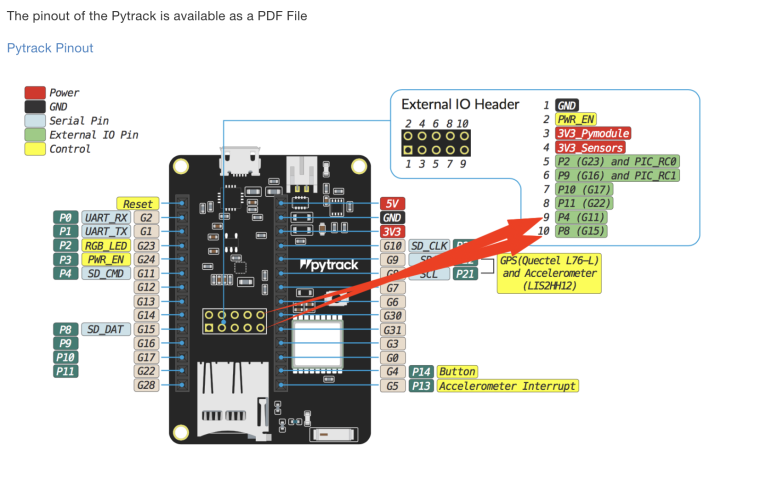
\includegraphics[width=\linewidth]{images/pytrack-external-gpio.png}
    \caption{Fig. 5.1.1: PyTrack-Ext-GPIO}
  \end{subfigure}
  \begin{subfigure}[b]{0.45\linewidth}
    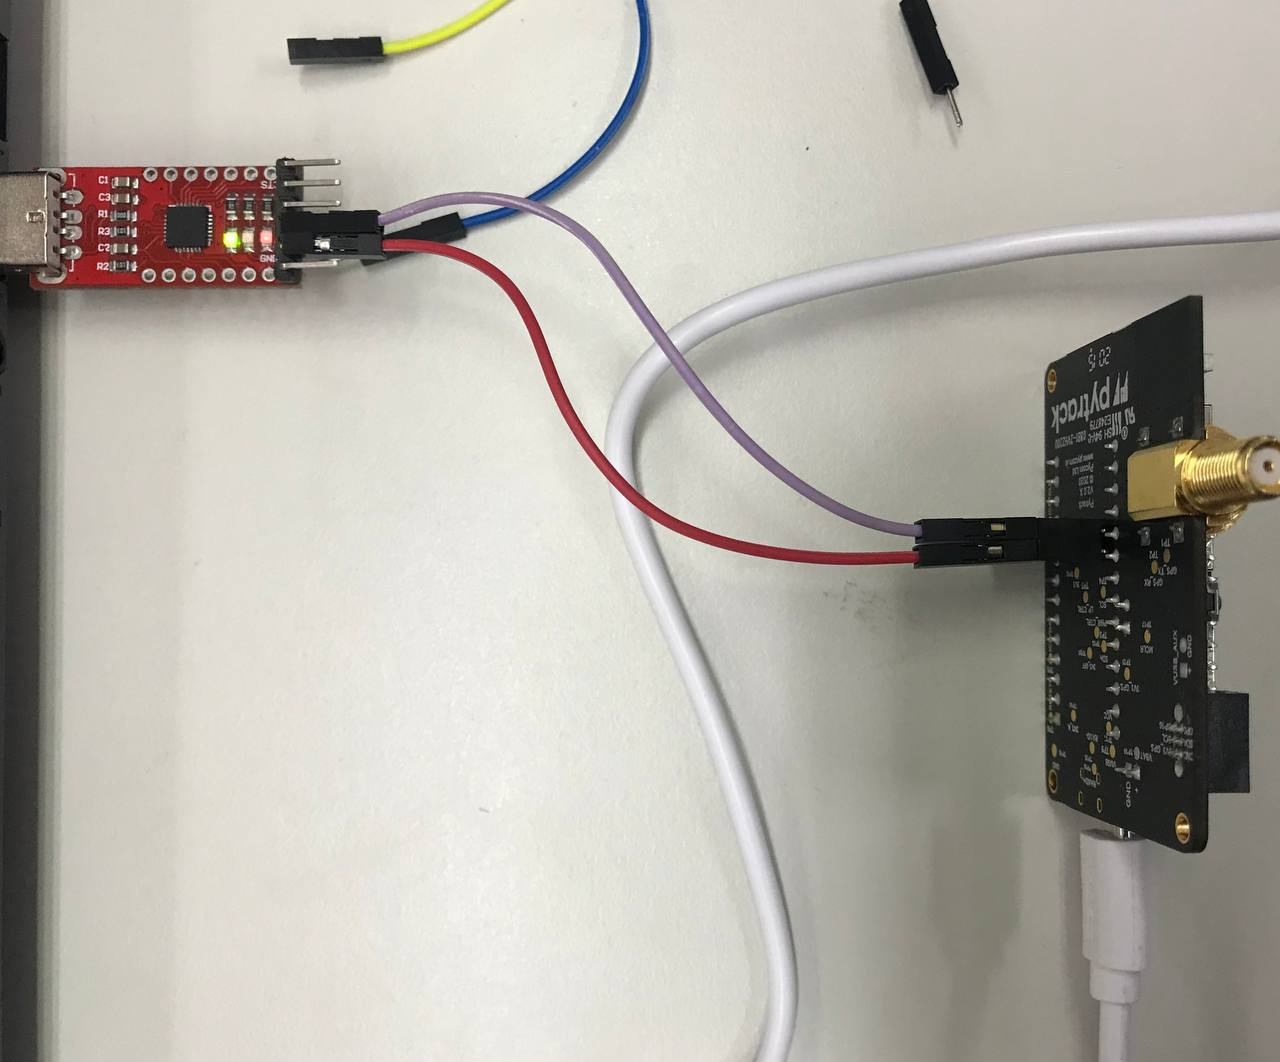
\includegraphics[width=\linewidth]{images/pytrack-external-gpio-2.png}
    \caption{Fig. 5.1.2: PyTrack-Ext-GPIO}
  \end{subfigure}
\end{figure}

\subsubsection{Carga de programas}

Con esto listo, solo resta cargar los programas de prueba en ambas placas, los cuales se pueden encontrar en el repositorio
\begin{itemize}
\item \path{../uart/PyCom/write_data_to_smt32.py} para enviar datos desde la \textit{PyCom} a la \textit{SMT32}.
\item \path{../uart/SMT32F4/uart_recieve/src} ahí se encuentran los archivos a compilar para la \textit{SMT32}, se recomienda abrir todo el workspace y compilar desde la herramienta.
\end{itemize}

\subsubsection{Conexionado}

Por último solo queda realizar el conexionado para obtener la siguiente topología, en la cúal la \textit{PyCom} enviará datos a ser leídos por la \textit{SMT32}. 

\begin{enumerate}
  \item PC1 a STM32 [Fig. 5.1.3].
  \item STM32 a Pycom  [Fig. 5.1.4].
  \item Pycom a PC2 [Fig. 5.1.5].
\end{enumerate}

Entonces solo queda, desde la \textit{PC1}, enviar información a la \textit{STM32}, la cuál se la comunicará con la \textit{PyCom} quién la leerá y los resultados pordrán ser validados en la \textit{PC2}.

\begin{figure}[ht]
  \centering
  \begin{subfigure}[b]{0.45\linewidth}
    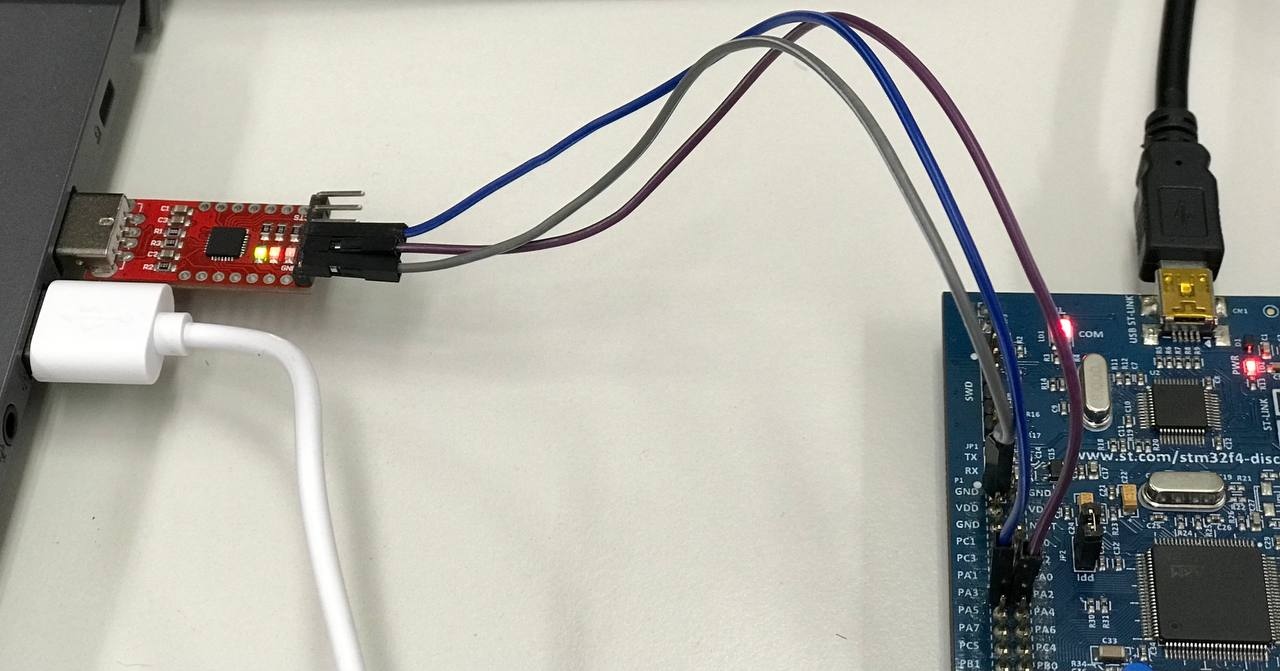
\includegraphics[width=\linewidth]{images/SMT32-PyCom-1.png}
    \caption{Fig. 5.1.3: PC1 a STM32}
  \end{subfigure}
  \begin{subfigure}[b]{0.45\linewidth}
    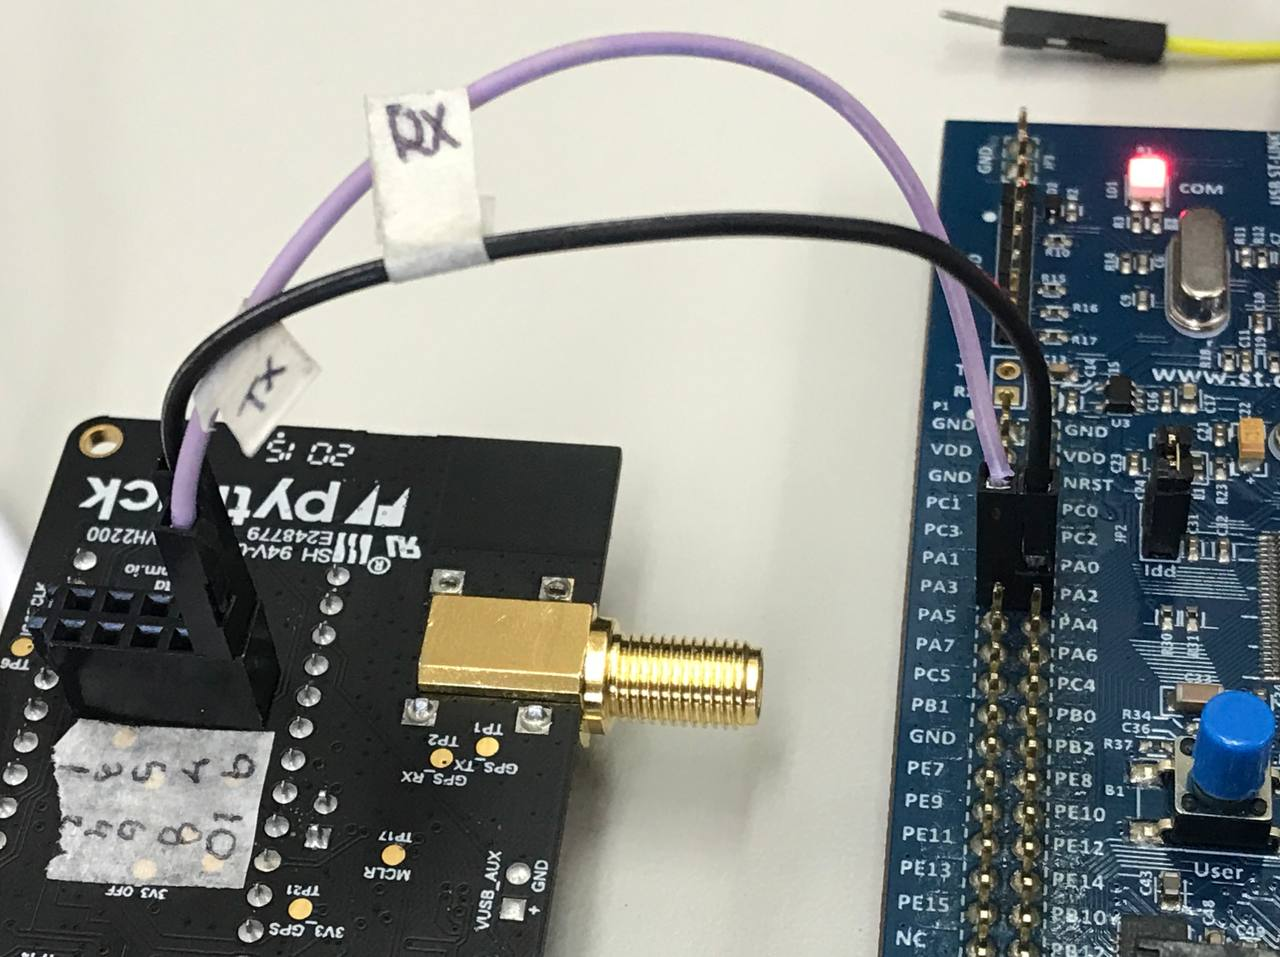
\includegraphics[width=\linewidth]{images/SMT32-PyCom-2.png}
    \caption{Fig. 5.1.4: STM32 a Pycom}
  \end{subfigure}
  \begin{subfigure}[c]{0.45\linewidth}
    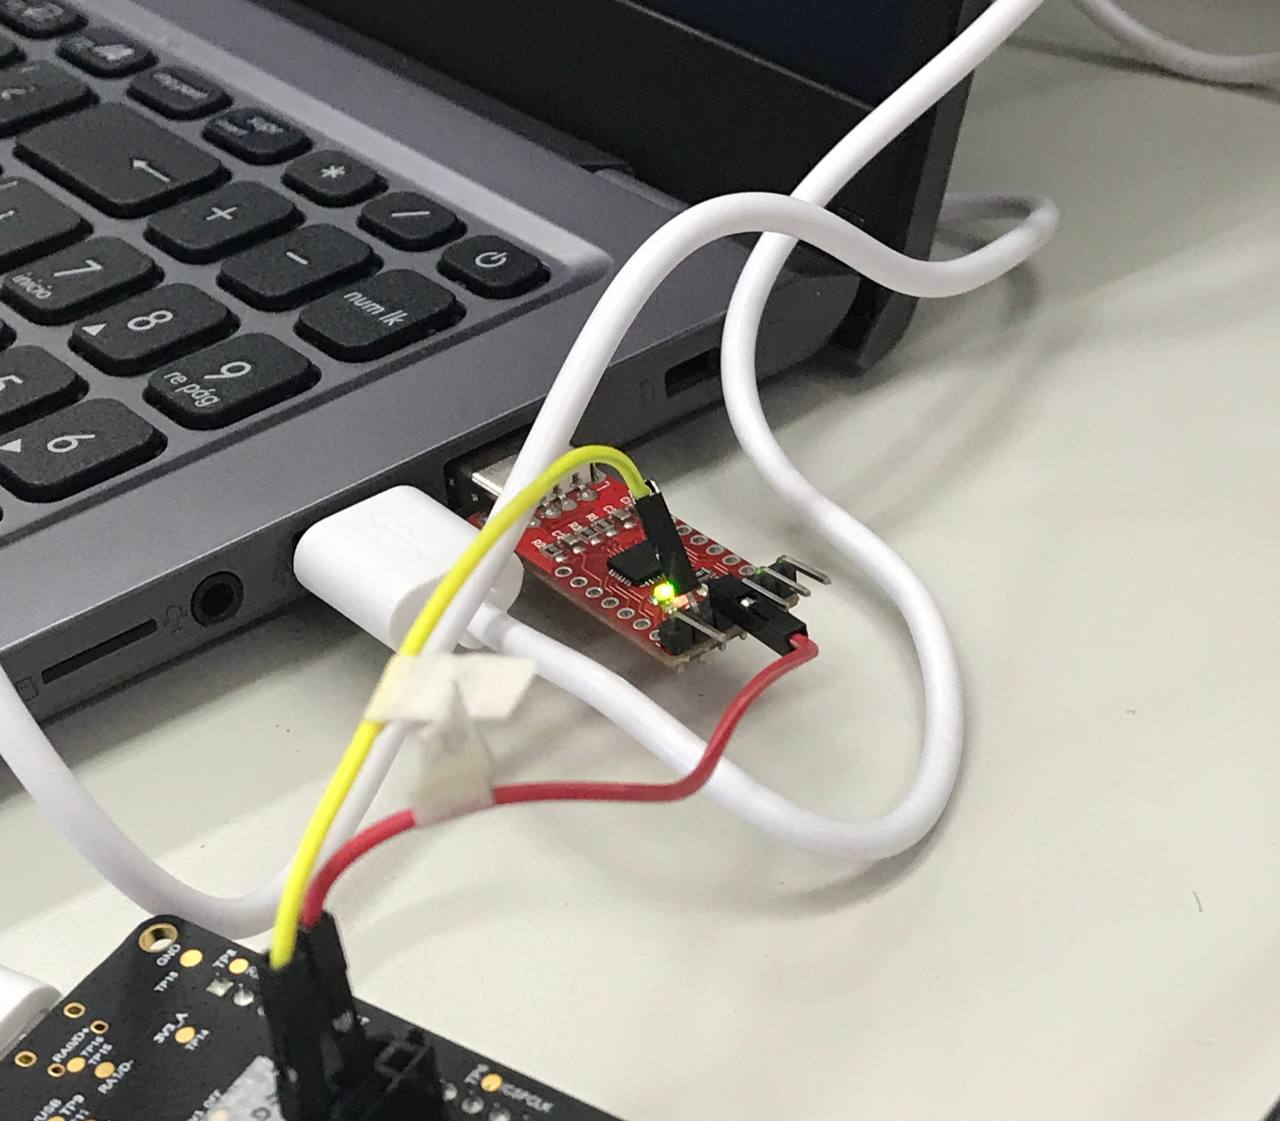
\includegraphics[width=\linewidth]{images/SMT32-PyCom-3.png}
    \caption{Fig. 5.1.5: Pycom a PC2}
  \end{subfigure}
\end{figure}

\subsection{DJI SDK}
La investigación sobre el \textit{SDK} del drone nace como respuesta a la oportunidad de montar payloads sobre \textit{UAV}. Tener cargas útiles sobre el drone es de una gran útilidad dado que utilizando \href{https://www.dji.com/d-rtk-2}{\textit{D-RTK2}} se pueden obtener datos de alta precisión a través del GPS del mismo, en tiempo real.

Algunas de las aplicaciones que podrían resultar de estas implementacio-nes son:
\begin{itemize}
  \item \textbf{Recolección de datos de multinodos}, en sistemas con multinodos que recopilan información, el drone puede ser una excelente opción para planificar rutas he ir recolectando e indicando a donde redireccionar los datos al mismo tiempo.
  \item \textbf{Inspección de redes de alta tensión}, permite encontrar defectos en las powerlines desde una distancia segura.
  \item \textbf{Agricultura de precisión}, ya sea para la detección de plagas, male-zas, monitorear rendimientos, intervenir en sectores específicos del cul-tivo de manera inmediata, etc.
  \item \textbf{Minería}, para inspeccionar cañerías de gas o combustible con lasers de detección de fugas.
  \item \textbf{Combate contra incendios}, se podría equipar con cámaras especiales con zoom óptico para identificar focos de fuego, planear estrategias y reconocer situaciones peligrosas.
  \item \textbf{Seguridad}, se podría utilizar para patrullaje y monitoreo de zonas conflictivas o díficiles de cubrir, como por ejemplo las fronteras.
\end{itemize}

\subsubsection{Módulos del SDK de DJI}
Ahora se adjuntarán los distintos módulos que existen el el SDK de payloads provisto por DJI, estos son los que abrirán las puertas a nuevas aplicaciones, los mismos se clasifican en dos grandes subsecciones, \textit{Basic Function} o \textit{Advanced Function}.

\begin{figure}[ht]
  \centering
  \begin{subfigure}[a]{1\linewidth}
    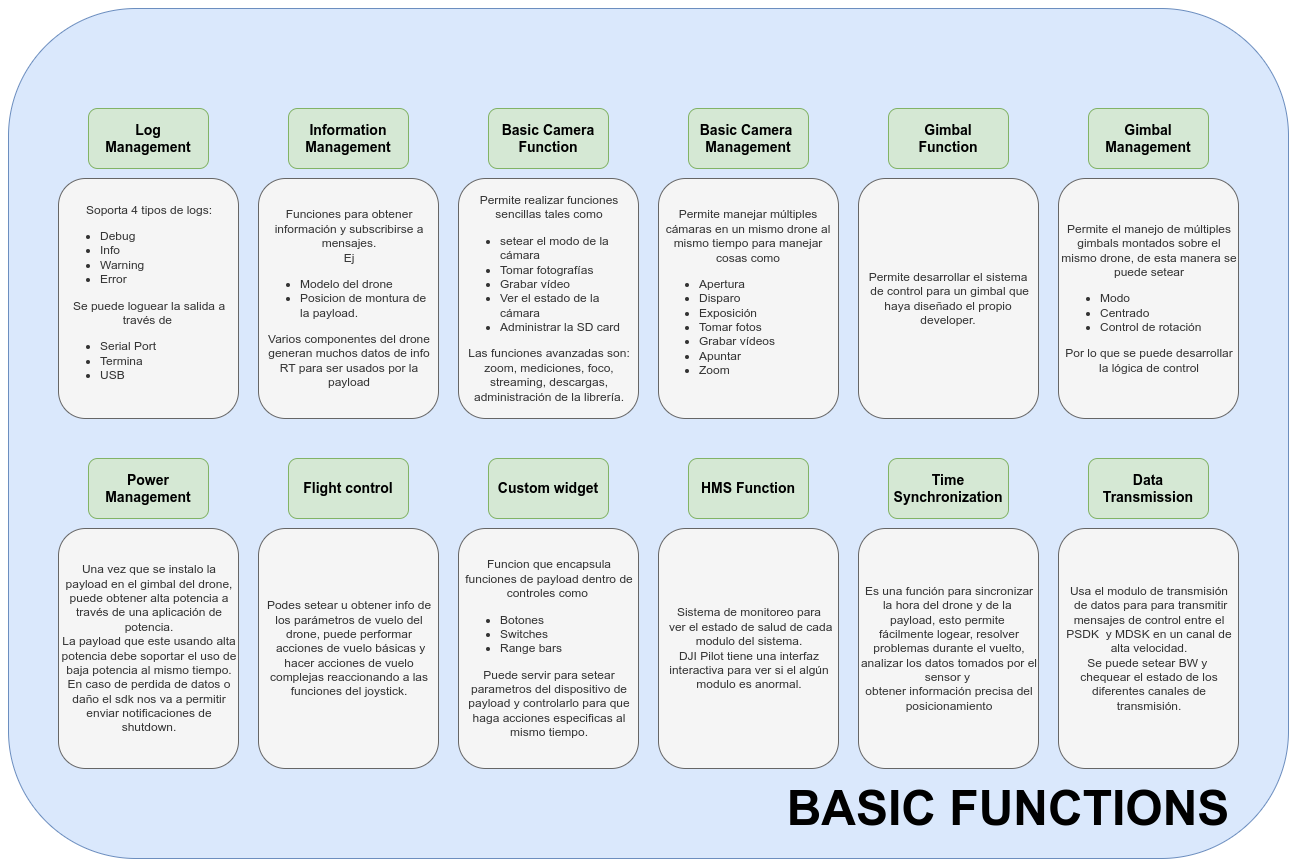
\includegraphics[width=\linewidth]{images/basic_function.png}
    \caption{Fig. 5.2.1: Basic Functions}
  \end{subfigure}
  \begin{subfigure}[b]{1\linewidth}
    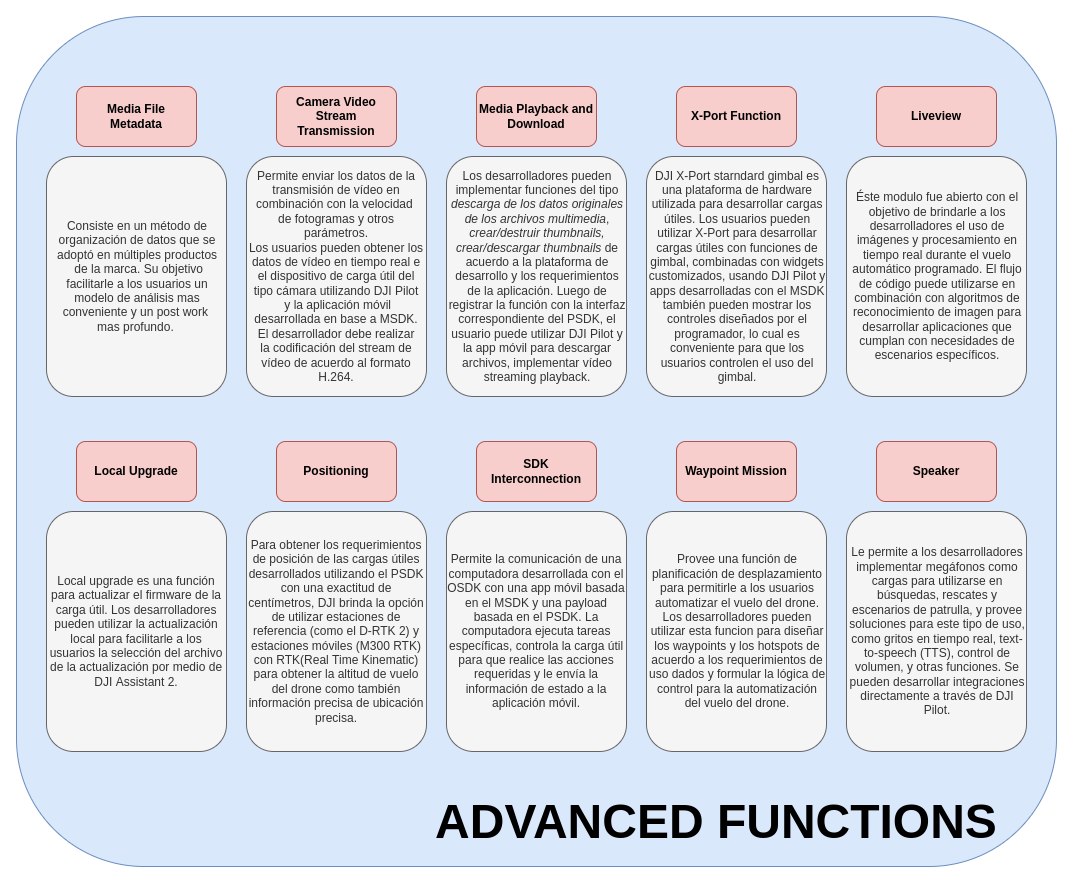
\includegraphics[width=\linewidth]{images/advanced_function.png}
    \caption{Fig. 5.2.1: Advanced Functions}
  \end{subfigure}
\end{figure}

\subsection{PyCom-CustomLogger}
Dado que el logger proporcionado por la librería de micropython es bastante limitado surgió la necesidad de implementar un logger genérico que nos permita visualizar la información obtenida por el drone de la mejor manera posible. Esto no es algo menor, ya que varias de las potenciales aplicaciones que tine nuestro \textit{UAV} consiste en la obtención y relevamiento de datos.

\subsubsection{Conexión a internet y servidor NTP}
Para la construcción del \textit{CustomLogger} lo primero que debimos implementar fue un módulo para el soporte del protocolo \href{https://es.wikipedia.org/wiki/Network_Time_Protocol}{\textit{NTP}} ya que es fundamental tener la hora en la que suceden los eventos que se quieren registrar. Para lo cual se creo un \href{https://github.com/sofia-am/DJI_Payload_Development/blob/main/log/micropython/lib/us_ntp.py}{módulo en python} que primero se conecta a internet, para luego poder sincronizarse utilizando el servidor \textit{NTP} de google.

\subsection{Logger}
Para realizar el logger nos basamos principalmente en el módulo que ya existía para micropython, luego le fuimos realizando las modificaciones pertinentes, de esta manera cada vez que se quiere registrar un evento se debe llamar a la función \textit{log} de la siguiente manera: \textbf{Logger.info("Mensaje a registrar")}, los tipos de logs soportados son:
\begin{itemize}
  \item debug (color gris)
  \item info (color verde)
  \item warning (color amarillo)
  \item error (color rojo)
  \item critical (color rojo)
  \item exception (color rojo)
\end{itemize}
El log es circular, con un tamaño máximo por defecto de 1Gb (parametrizable), es decir, a partir del Gb de información comienza a sobreescribirse.

\begin{figure}[ht]
  \centering
  \begin{subfigure}[a]{1\linewidth}
    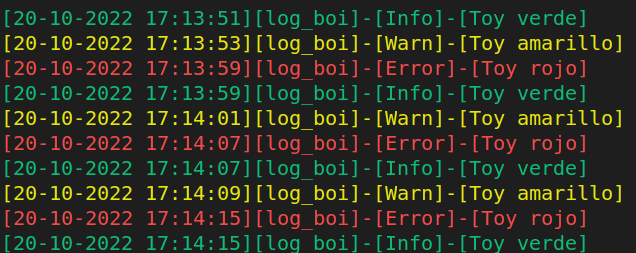
\includegraphics[width=\linewidth]{images/PyCom-Logger.png}
    \caption{Fig. 5.4.1: CustomLogger}
  \end{subfigure}
\end{figure}

\subsection{Post-Flight Processor}
Mientras se esperaba por la llegada de nuevos componentes, se decidió realizar una prueba de concepto para la implementación de un \textit{Post-Flight Processor}, un script que permita mergear los datos obtenidos (post vuelo) por el drone, con los que se obtengan de los sensores externos de nuestra payload.

\subsubsection{DJI Logs}
Los logs post vuelo de DJI vienen encriptados, por lo que lo primero que se debe hacer es desencriptarlos, para esto se utiliza \href{https://www.phantomhelp.com/logviewer/upload/}{\textit{PhantomHelpLogViewer}}, simplemente se siguen los pasos para subir el archivo obtenido del comando del drone, y una vez procesado descargar el \textit{.csv} obtenido.
De este archivo la información que nos interesaría obtener a priori es 
\begin{itemize}
  \item Date
  \item Lat
  \item Lon
  \item Height
  \item Altitude
\end{itemize}

\subsubsection{CSV Handler}
El primer paso para trabajar con los logs obtenidos del drone fue crear un handler, que nos permita leer el archivo \textit{.csv}, obtener los datos de interés, con ellos crear un \textit{DataFrame} apoyandonos con \href{https://pandas.pydata.org/}{\textit{Pandas}}.
Dadas las particularidades de como se guardan las fechas en los logs, y la necesidad de que sean idénticas a las que obtenemos con nuestro \textit{CustomLogger} en la \textit{PyCom}, se necesitaron múltiples funciones auxiliares para el manejo de strings, la mayoría se resuelve con programación funcional (lambdas, maps, etc), además se implementaron test unitarios para asegurarnos del correcto funcionamiento de las mismas.

Se puede consultar el código para este módulo en \href{https://github.com/sofia-am/DJI\_Payload\_Development/blob/main/log/post\_flight\_logger\_processor/src/csv\_handler.py}{\textit{csv\_handler.py}}.

\subsubsection{Implementación del procesador}
El funcionamiento conceptualmente no es demasiado complejo, se trata de obtener todas las fechas del archivo \textit{.log} de la payload, esto se consigue utilizando una RegEx, luego con esos datos como input consultamos a el \textit{DataFrame} que obtuvimos de los logs de \textit{DJI} obteniendo así la información de ese instante, finalmente se escribe un nuevo log con los resultados [Fig 5.5.2].

\begin{figure}[ht]
  \centering
  \begin{subfigure}[a]{1\linewidth}
    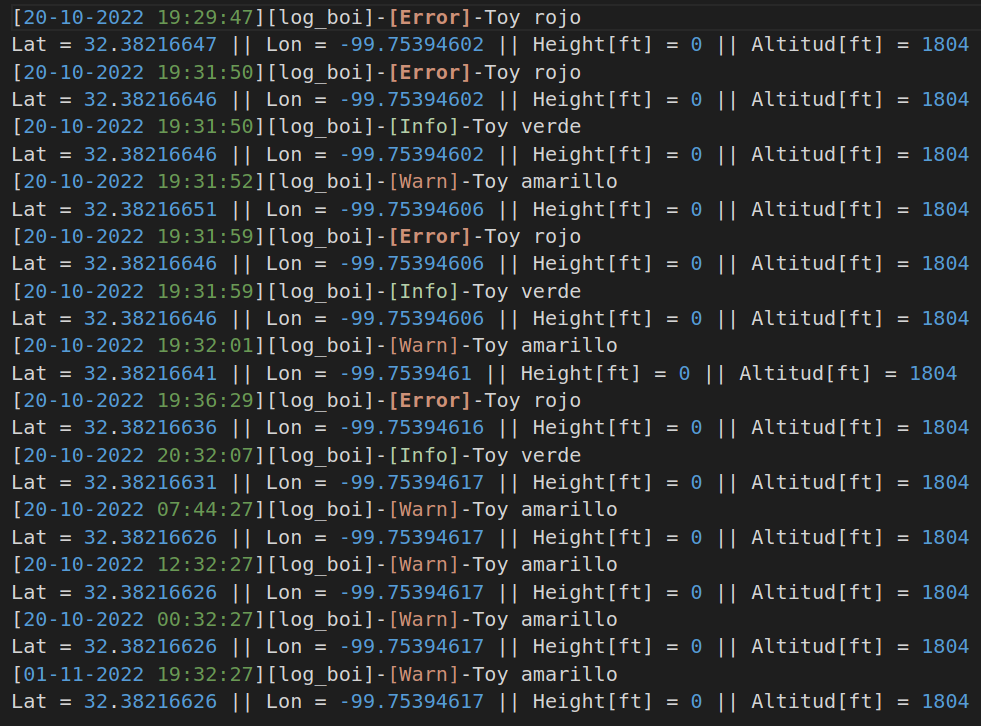
\includegraphics[width=\linewidth]{images/post-flight-processor.png}
    \caption{Fig. 5.5.2: PostFlight-Processor}
  \end{subfigure}
\end{figure}

\subsection{Análisis Robomaster}

\newpage
\begin{thebibliography}{9}
\bibitem{uart} \url{https://www.rohde-schwarz.com/lat/productos/prueba-y-medicion/essentials-test-equipment/digital-oscilloscopes/entendiendo-el-uart_254524.html} 


\end{thebibliography}
\end{document}